% !TEX root =  master.tex
\chapter{Einleitung}
\section{Motivation und Zielsetzung}
In den letzten Jahren hat Computertechnologie rasant an Leistungsfähigkeit und Funktionsumfang zugenommen.
Längst sind Computer oder Mobilgeräte nicht mehr aus dem Alltag wegzudenken.
Umso wichtiger ist es, diese Technologien sinnvoll in die Tätigkeiten von Menschen zu integrieren und durch diesen einen wertvollen Mehrwert zu generieren.
Immer mehr Themenbereiche sind und müssen digitalisiert werden.

Zum Anlass des aktuellen Weltgeschehens sehen wir die Notwendigkeit, solche Technologien auch in den Hochschul-Kontext einzubringen.
Die aktuell \enquote{Corona-Krise} hat extreme Auswirkungen und macht sich in vielen Bereichen bemerkbar.
Mit einer der Bereiche, die am stärksten betroffen sind, ist das Bildungswesen.
So sind bereits im April 2020 die Schulen von 192 Ländern geschlossen worden.\autocite[S. 845]{Donohue2020}
Die geänderten Anforderungen an Schüler und Studenten durch neue Konzepte wie \enquote{Home-Schooling} erfordern auch Anpassungen im Hochschulkontext.

Mit der von uns entwickelten Anwendung beabsichtigen wir die entstandene Distanz zwischen Studenten und Dozenten zu verringern. 
Mithilfe der Webanwendung möchten wir allen Studierenden und Dozierenden an der DHBW eine Möglichkeit bieten, ihren Hochschulalltag zu organisieren. 
Unsere Vision ist, dass unsere Anwendung einen Mehrwert für Studierende und Dozierende generiert wird.
Daher sollen möglichst alle Aufgaben des Hochschulalltags mit unserer Webanwendung unterstützt werden. 
Im Rahmen dieses Moduls soll ein Grundstein gelegt werden, auf dem weitere Entwicklung aufgebaut werden kann und auch soll.

\clearpage
\section{Aufbau der Arbeit} % TODO: Dieses Kapitel anpassen
In dieser Arbeit werden zunächst die Anforderungen an eine solche Anwendung betrachtet.
Dafür wird als erstes das Thema dieses Projektes abgegrenzt, um den Fokus unseres Vorhabens ausführlich darzustellen.
Anschließend wird der aktuelle Ist-Zustand analysiert, um herauszufinden wie Studenten und Dozenten am besten unterstützt werden können.
Ziel ist es festzustellen, welche funktionalen und welche nicht-funktionalen Anforderungen durch die Anwendung erfüllt werden sollten.

Basierend auf den festgestellten Anforderungen wird ein Konzept ausgearbeitet.
Im Konzept wird nicht nur auf die Funktionalitäten, wie sie Nutzer verwenden können eingegangen, sondern auch auf die technischen Hintergründe.

Anschließend wird die Umsetzung des Konzeptes beschrieben.
Der Fokus liegt dabei auf der Schaffung von Transparenz bezogen auf die verarbeiteten Daten.
Als letztes Hauptkapitel wird die Nutzung der Anwendung durch dritte Personen wie Studenten und Dozenten beschrieben.
% TODO: Hier noch schauen. Soll die Nutztung tatsächlich als eigenes Kapitel geschrieben werden? ist das nicht schon in der Konzeption, und Umsetzung?

Das Nutzerhandbuch stellt eine eindeutige und verständliche Nutzeranleitung dar.
Mithilfe dieser werden alle Funktionalitäten der Endanwendung erklärt.
% TODO: Das auchnochmal reinschauen.   Brauchen wir wirklich ein Kapitel in dem nochmal die ganzen Anforderungen validiert werden? Das steht doch dann auch schon in Konzeption + Umsetzung ?
% TODO: Hier nochmal sätze bauen

Den Abschluss der Dokumentation ist die Zusammenfassung.
Diese besteht aus zwei Teilen.
Das Fazit betrachtet das Projekt als Ganzes und vergleicht die schlussendliche Form mit den in der Einleitung hervorgestellten Zielen. Damit werden alle Tätigkeiten innerhalb dieses Projekts abgerundet abgeschlossen dargestellt.
Anschließend wird ein Ausblick hervorgestellt, an welchen Stellen Folgeprojekte aufbauen können. Was wir aus aktueller Sicht als sinnvoll betrachten, auf was dabei zu achten ist und was vermieden werden sollte.


% TODO: Hier stand noch was drin, dass auch Datenschutz sachen und so beschrieben. Das weiß ich nicht. Das kann man hier reinschreiben, wenn wir das tatsächlich machen. 

\clearpage
\section{Vorgehen}
Wir haben uns in dieser stark an das Vorgehen des Framworks Scrum gehalten. Scrum ist ein Vorgehensmodell aus der agilen Softwareentwicklung und dem agilen Projektmanagement. Das Framework vertritt die weit verbreitete Meinung, dass Softwareprojekte nicht im Voraus planbar sind, weshalb Planung nur schrittweise und durch immer weitere Verfeinerungen erfolgen sollte. Scrum basiert auf folgenden vier Grundwerten:
\begin{center}
	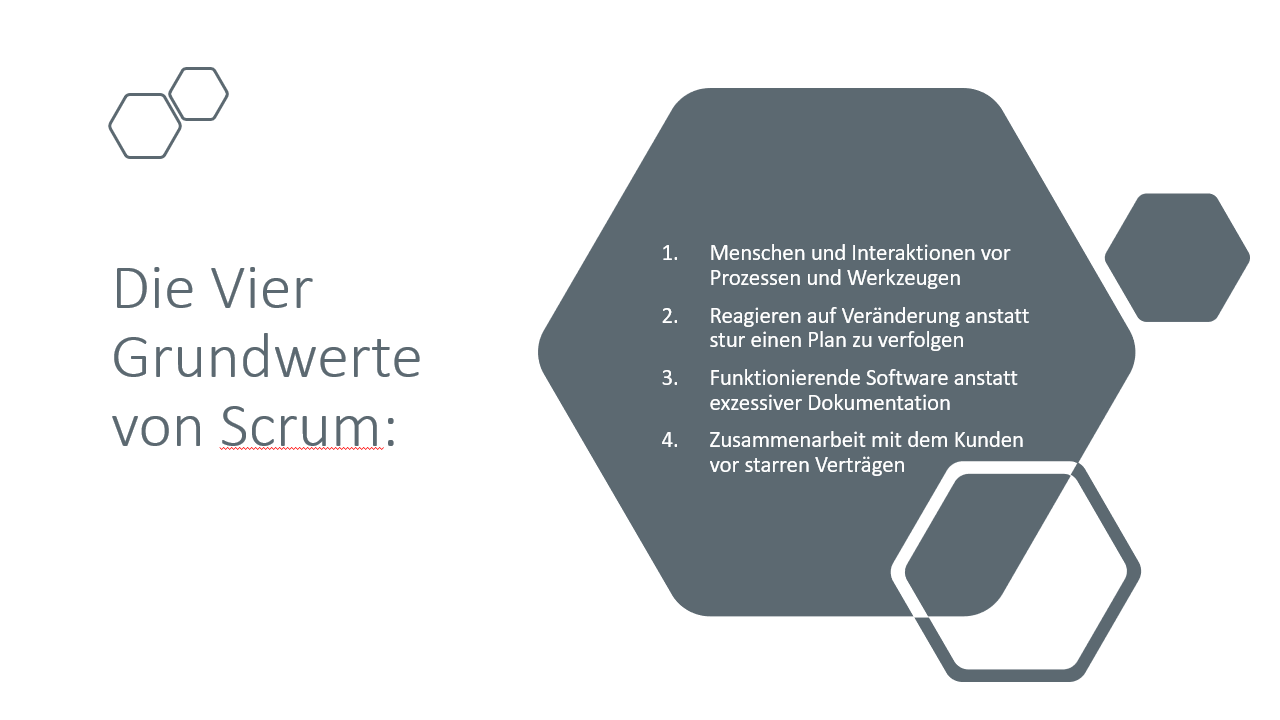
\includegraphics[width=14cm, keepaspectratio]{img/4Scrum} 
\end{center}

Wie bereits in der Beschreibung angeklungen ist, ist Scrum ein iteratives Vorgehen. Das beutetet, es gibt regelmäßige Arbeitsroutinen, die immer wiederholt werden. Ein solcher Abschnitt wird in Scrum Sprint genannt. Ein Sprint besteht aus folgenden festen Ritualen:
\begin{center}
	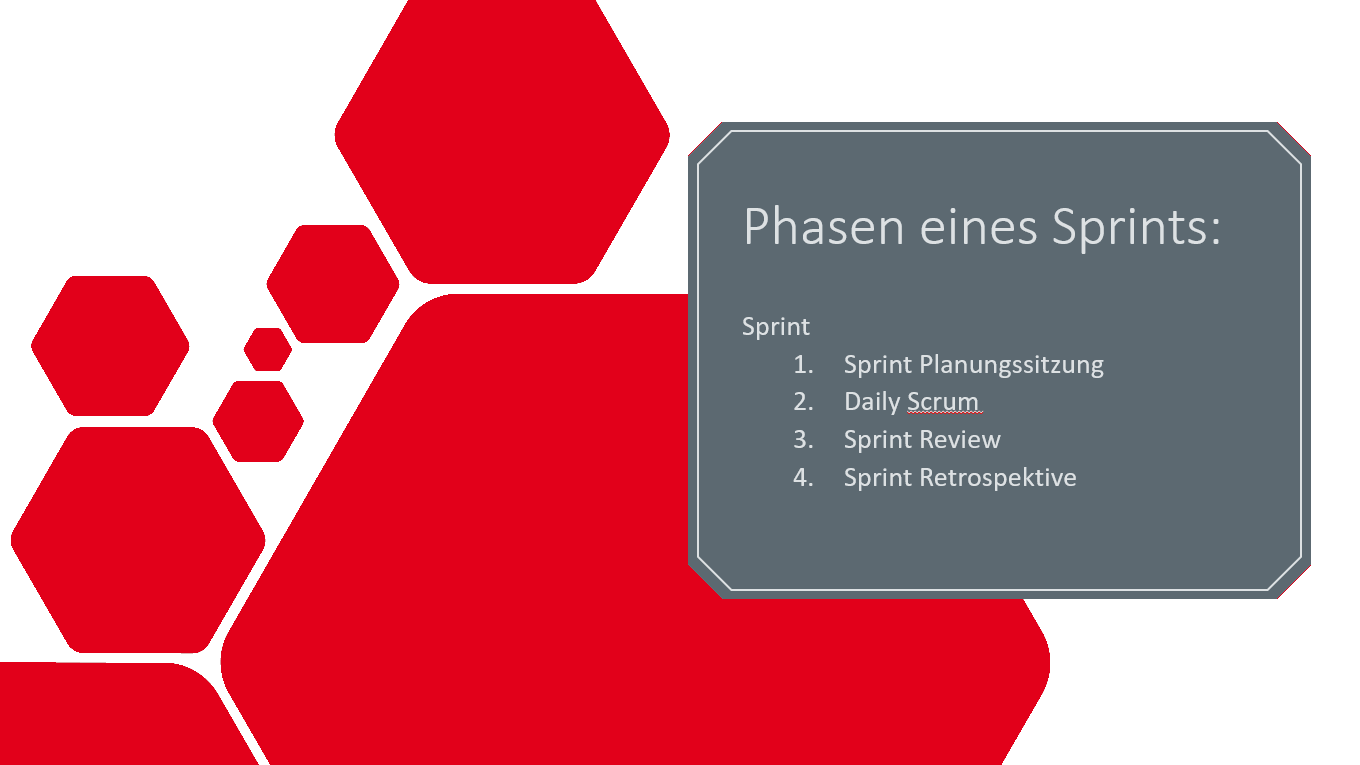
\includegraphics[width=14cm, keepaspectratio]{img/5Scrum} 
\end{center}


Wir haben uns für die Dauer eines Sprints von 2 Wochen entschieden. Zu Beginn eines jeden Sprints fand eine virtuekke Planungssitzung statt, bei der die anstehenden Aufgaben bezüglich ihrer Komplexität geschätzt wurden und gemeinsam diskutiert wurde, welche im Sprint erledigt und somit in das Sprint Backlog aufgenommen werden müssen. Da sich die Ausarbeitung dieses Projektes über zwei Theoriesemester und eine Praxisphase zog, in der wir auch unsere Bachelorarbeiten geschrieben haben, hatten wir uns schnell für das Pull Prinzip entschieden. Das bedeutet im Wesentlichen nur, dass jeder sich selbst aufgaben nimmt und nicht zentral von einer Person zugewiesen bekommt. So wollten wir sicherstellen, dass jeder von uns zu jederzeit ein machbares Arbeitspensum erreichen kann, bei dem wir sowohl den Anforderungen des Projektes als auch den Anforderungen der geschriebenen Klausuren und unseren Bachelorarbeiten gerecht werden konnten. Die anfallenden Aufgaben haben wir in Arbeitspackete als Issues in unserem github Projekt angelegt, über das wir auch unseren Code versionieren und Deployments mittels github Actions anstoßen. Ein Issue kann prinzipiell jedes Team Mitglied erstellen. Da innerhalb eines Sprints der Umfang und die Inhalte jedoch geschützt sind und somit nicht verändert werden, war sichergestellt, dass wir spätestens im nächsten Sprint Planning über diese Issues diskutieren, wenn es um die Frage ging, welche Inhalte im nächsten Sprint umgesetzt werden sollten. 

 Das Daily Scrum stellt einen täglichen Termin da, bei dem der aktuelle Stand der einzelnen Teammitglieder durchgegangen wird und gemeinsam über Probleme und Impediments gesprochen wird. Aufgrund des langen Projektzeitraums und der oben genannten Gründe haben wir uns gegen ein tägliches Daily entschieden. Da wir in der Gruppenkonstellation häufig zusammenarbeiten sind wir auch außerhalb des Sprintplannings regelmäßig in Kontakt und können so auch zielgerichteter und bedarfsgesteuert Themen in großer oder kleiner Gruppe diskutieren. 
 
 Ein Sprint Review fand am Ende eines jeden Sprints, also alle 14 Tage statt. Dabei werden die umgesetzten Inhalte kurz der Gruppe vorgestellt und Feedback der Teammitglieder eingeholt. So können schnell fachliche Missverständnisse entdeckt und behoben werden. Außerdem verbessert dieses vorgehen im Regelfall die Codequalität. Scrum sieht eigentlich vor, das in diesem Termin auch die Stakeholder eingebunden werden um Feedback der Auftraggeber frühestmöglich einholen zu können. Da dies aus Zeit und Ressourcen Gründen unrealistisch erschien, haben wir uns gemeinsam entschieden an dieser Stelle vom Prozess abzuweichen und nur die während den Vorlesungsstunden einberaumten Abstimmungen zu nutzen um die seit der letzten Abstimmung umgesetzten Features vorzustellen und Abzustimmen. Mit dieser Entscheidung haben wir uns auch commitet keine extra Sprint Retrospektive abzuhalten. Ziel dieses Termins ist es innerhalb des Teams zu schauen, wie der letzte Sprint lief und wie man die gemeinsame Arbeit verbessern kann. Dies ist als extra Termin geplant, weil er dem Sprintteam gehört und nur intern bleiben soll. Hier gibt es in der Literatur sehr viele Beispiele auf die so genannte Las Vegas regel - \enquote{Alles was in Vegas passiert bleibt in Vegas}. Da bereits unsere Sprint Reviews nur innerhalb des Teams abgehalten wurden, beschlossen wir nicht mehr Zeit in einem extra Termin veranschlagen zu müssen sondern in unser speziellen Konstellation die beiden Termine nacheinander mit einem fließenden Übergang abhalten zu können. 
 
Diesen Prozess verfolgten wir nach der ersten Vorlesung, die wir dazu nutzten, uns einen Überblick über die eigentliche Aufgabenstellung, das Themengebiet und die Arbeitspakete zu verschaffen. 